\let\negmedspace\undefined
\let\negthickspace\undefined
\documentclass[journal,12pt,twocolumn]{IEEEtran}
\usepackage{gensymb}
\usepackage{amssymb}
\usepackage[cmex10]{amsmath}
\usepackage{amsthm}
\usepackage[export]{adjustbox}
\usepackage{bm}
\usepackage{longtable}
\usepackage{enumitem}
\usepackage{mathtools}
 \usepackage{tikz}
\usepackage[breaklinks=true]{hyperref}
\usepackage{listings}
\usepackage{color}                                            %%
\usepackage{array}                                            %%
\usepackage{longtable}                                        %%
\usepackage{calc}                                             %%
\usepackage{multirow}                                         %%
\usepackage{hhline}                                           %%
\usepackage{ifthen}                                           %%
\usepackage{lscape}     
\usepackage{multicol}
 \usepackage{enumerate}
\DeclareMathOperator*{\Res}{Res}
\renewcommand\thesection{\arabic{section}}
\renewcommand\thesubsection{\thesection.\arabic{subsection}}
\renewcommand\thesubsubsection{\thesubsection.\arabic{subsubsection}}
\renewcommand\thesectiondis{\arabic{section}}
\renewcommand\thesubsectiondis{\thesectiondis.\arabic{subsection}}
\renewcommand\thesubsubsectiondis{\thesubsectiondis.\arabic{subsubsection}}
\hyphenation{op-tical net-works semi-conduc-tor}
\def\inputGnumericTable{}                                 %%
\lstset{
frame=single, 
breaklines=true,
columns=fullflexible
}
\begin{document}
\newcommand{\BEQA}{\begin{eqnarray}}
\newcommand{\EEQA}{\end{eqnarray}}
\newcommand{\define}{\stackrel{\triangle}{=}}
\newcommand*\circled[1]{\tikz[baseline=(char.base)]{
    \node[shape=circle,draw,inner sep=2pt] (char) {#1};}}
\bibliographystyle{IEEEtran}
\providecommand{\mbf}{\mathbf}
\providecommand{\pr}[1]{\ensuremath{\Pr\left(#1\right)}}
\providecommand{\qfunc}[1]{\ensuremath{Q\left(#1\right)}}
\providecommand{\sbrak}[1]{\ensuremath{{}\left[#1\right]}}
\providecommand{\lsbrak}[1]{\ensuremath{{}\left[#1\right.}}
\providecommand{\rsbrak}[1]{\ensuremath{{}\left.#1\right]}}
\providecommand{\brak}[1]{\ensuremath{\left(#1\right)}}
\providecommand{\lbrak}[1]{\ensuremath{\left(#1\right.}}
\providecommand{\rbrak}[1]{\ensuremath{\left.#1\right)}}
\providecommand{\cbrak}[1]{\ensuremath{\left\{#1\right\}}}
\providecommand{\lcbrak}[1]{\ensuremath{\left\{#1\right.}}
\providecommand{\rcbrak}[1]{\ensuremath{\left.#1\right\}}}
\theoremstyle{remark}
\newtheorem{rem}{Remark}
\newcommand{\sgn}{\mathop{\textbf{sgn}}}
\providecommand{\abs}[1]{\left\vert#1\right\vert}
\providecommand{\res}[1]{\Res\displaylimits_{#1}} 
\providecommand{\norm}[1]{\left\lVert#1\right\rVert}
%\providecommand{\norm}[1]{\lVert#1\rVert}
\providecommand{\mtx}[1]{\mathbf{#1}}
\providecommand{\mean}[1]{E\left[ #1 \right]}
\providecommand{\fourier}{\overset{\mathcal{F}}{ \rightleftharpoons}}
%\providecommand{\hilbert}{\overset{\mathcal{H}}{ \rightleftharpoons}}
\providecommand{\system}{\overset{\mathcal{H}}{ \longleftrightarrow}}
	%\newcommand{\solution}[2]{\textbf{Solution:}{#1}}
\newcommand{\solution}{\noindent \textbf{Solution: }}
\newcommand{\cosec}{\,\text{cosec}\,}
\providecommand{\dec}[2]{\ensuremath{\overset{#1}{\underset{#2}{\gtrless}}}}
\newcommand{\myvec}[1]{\ensuremath{\begin{pmatrix}#1\end{pmatrix}}}
\newcommand{\mydet}[1]{\ensuremath{\begin{vmatrix}#1\end{vmatrix}}}
\newcommand*{\permcomb}[4][0mu]{{{}^{#3}\mkern#1#2_{#4}}}
\newcommand*{\perm}[1][-3mu]{\permcomb[#1]{P}}
\newcommand*{\comb}[1][-1mu]{\permcomb[#1]{C}}
%\numberwithin{equation}{subsection}
\makeatletter
\@addtoreset{figure}{problem}
\makeatother
\let\StandardTheFigure\thefigure
\let\vec\mathbf
%\renewcommand{\thefigure}{\theproblem}
\def\putbox#1#2#3{\makebox[0in][l]{\makebox[#1][l]{}\raisebox{\baselineskip}[0in][0in]{\raisebox{#2}[0in][0in]{#3}}}}
     \def\rightbox#1{\makebox[0in][r]{#1}}
     \def\centbox#1{\makebox[0in]{#1}}
     \def\topbox#1{\raisebox{-\baselineskip}[0in][0in]{#1}}
     \def\midbox#1{\raisebox{-0.5\baselineskip}[0in][0in]{#1}}
\vspace{3cm}
\title{Assignment}
\author{Anshul Sangrame\\CS21BTECH11004
	\thanks{}
}

% make the title area
\maketitle

\newpage

%\tableofcontents

\bigskip

%\renewcommand{\thefigure}{\theenumi}
%\renewcommand{\thetable}{\theenumi}
%\renewcommand{\theequation}{\theenumi}

\section{Uniform Random Numbers}

\textbf{1.1: }Generate $10^6$ samples of U using a C program and save into a file called uni.dat .

    \solution
    
Download the following files,
\begin{lstlisting}
wget https://github.com/Anshul-Sangrame/AI1110/blob/main/Assignment/solution/1/coeffs.h
wget https://github.com/Anshul-Sangrame/AI1110/blob/main/Assignment/solution/1/1_1.c
\end{lstlisting}

Execute the above files using code,
\begin{lstlisting}
gcc 1_1.c -lm
./a.out
\end{lstlisting}

\textbf{1.2: }Load the uni.dat file into python and plot the empirical CDF of U using the samples
in uni.dat. The CDF is defined as
\begin{align*}
    F_U(x) = Pr(U \leq x)
\end{align*}

    \solution
    
Download the following files
\begin{lstlisting}
wget https://github.com/Anshul-Sangrame/AI1110/blob/main/Assignment/solution/1/1_2.py
\end{lstlisting}

Execute the code using command
\begin{lstlisting}
python3 1_2.py
\end{lstlisting}

Plot \ref{fig:1.3} is obtained,
\begin{figure}[!ht]
	\centering
	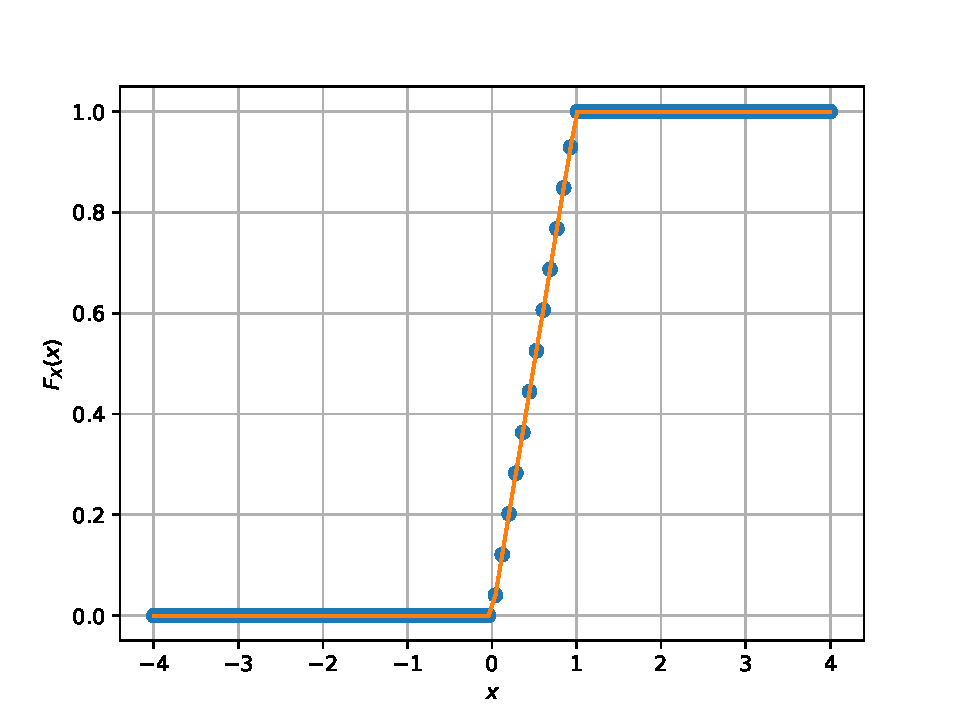
\includegraphics[width=\columnwidth]{figs/uni_cdf.pdf}
	\caption{}
	\label{fig:1.3}
\end{figure}

\textbf{1.3: } Find a theoretical expression for $F_U(x)$.
	\solution
	
Pdf of Uniform distribution between [0,1] is given by,
\begin{align}
    f_U(x) = \begin{cases}
        1, & x \in [0,1] \\
        0, & \text{otherwise}
    \end{cases}
\end{align}

\begin{align}
    F_U(x) = \int_{-\infty}^{x} f_U(x) dx
\end{align}

Case-1: x $<$ 0,

\begin{align}
    F_U(x) &= \int_{-\infty}^{x} 0 dx \\
    &= 0
\end{align}

Case-2: x $\in$ [0,1],

\begin{align}
    F_U(x) &= \int_{-\infty}^{0} 0 dx + \int_{0}^{x} 1 dx\\
    &= x
\end{align}\

Case-3: x $>$ 1,

\begin{align}
    F_U(x) &= \int_{-\infty}^{0} 0 dx + \int_{0}^{1} 1 dx + \int_{1}^{x} 0 dx\\
    &= 1
\end{align}

Hence,
\begin{align}
    F_U(x) = \begin{cases}
    0, & x < 0 \\
    x, & x \in [0,1] \\
    1, & x > 1
    \end{cases}
\end{align}

\textbf{1.4: } The mean of U is defined as
\begin{align*}
    E[U] = \frac{1}{N} \sum_{i=1}^{N} U_i
\end{align*}
and its variance as
\begin{align*}
    \text{var}\sbrak{U} = E\sbrak{U- E\sbrak{U}}^2 
\end{align*}
Write a C program to find the mean and variance of U.

    \solution
    
Download the following files,
\begin{lstlisting}
wget https://github.com/Anshul-Sangrame/AI1110/blob/main/Assignment/solution/1/coeffs.h
wget https://github.com/Anshul-Sangrame/AI1110/blob/main/Assignment/solution/1/1_4.c
\end{lstlisting}

Execute the above files using code,
\begin{lstlisting}
gcc 1_4.c -lm
./a.out
\end{lstlisting}

The following result is obtained
\begin{align*}
    E\sbrak{U} &= 0.500007 \\
    \text{var}\sbrak{U} &= 0.083301
\end{align*}

\textbf{1.5: } Verify your result theoretically given Z that,
    \begin{align*}
        E[U^k] = \int_{-\infty}^{\infty} x^k dF_U(x)
    \end{align*}
	\solution
	
$F_U(x)$ for uniform distribution,
\begin{align}
    F_U(x) = \begin{cases}
    0, & x < 0 \\
    x, & x \in [0,1] \\
    1, & x > 1
    \end{cases}
\end{align}

\begin{align}
    E[U] &= \int_{-\infty}^{\infty} x dF_U(x) \\
    &= \int_{-\infty}^{0} 0 dx + \int_{0}^{1} x dx + \int_{1}^{\infty} 0 dx \\
    \label{eq: U}
    &= \frac{1}{2}
\end{align}

\begin{align}
    E[U^2] &= \int_{-\infty}^{\infty} x^2dF_U(x) \\
    &= \int_{-\infty}^{0} 0 dx + \int_{0}^{1} x^2 dx + \int_{1}^{\infty} 0 dx \\
    \label{eq: U^2}
    &= \frac{1}{3}
\end{align}

\begin{align}
    E[U-E[U]]^2 &= E[U^2] - [E[U]]^2
\end{align}

From Equation \eqref{eq: U} and \eqref{eq: U^2},
\begin{align}
    E[U-E[U]]^2 &= \frac{1}{3} - \brak{\frac{1}{2}}^2 \\
    &= \frac{1}{3} - \frac{1}{4} \\
    &= \frac{1}{12} \approx 0.083
\end{align}

\section{Central Limit Theorem}

\textbf{2.1: }Generate $10^6$ samples of the random variable
%
\begin{equation}
X = \sum_{i=1}^{12}U_i -6
\end{equation}
%
using a C program, where $U_i, i = 1,2,\dots, 12$ are  a set of independent uniform random variables between 0 and 1
and save in a file called gau.dat

    \solution
    
Download the following files,
\begin{lstlisting}
wget https://github.com/Anshul-Sangrame/AI1110/blob/main/Assignment/solution/1/coeffs.h
wget https://github.com/Anshul-Sangrame/AI1110/blob/main/Assignment/solution/2/2_1.c
\end{lstlisting}

Execute the above files using code,
\begin{lstlisting}
gcc 2_1.c -lm
./a.out
\end{lstlisting}

\textbf{2.2: }Load gau.dat in python and plot the empirical CDF of $X$ using the samples in gau.dat. What properties does a CDF have?

    \solution
    
Download the following files,
\begin{lstlisting}
wget https://github.com/Anshul-Sangrame/AI1110/blob/main/Assignment/solution/2/2_2.py
\end{lstlisting}

Execute the above file using code,
\begin{lstlisting}
python3 2_2.py
\end{lstlisting}

Plot \ref{fig:2.2} obtained is symmetric about (0,0.5)

\begin{figure}[!ht]
	\centering
	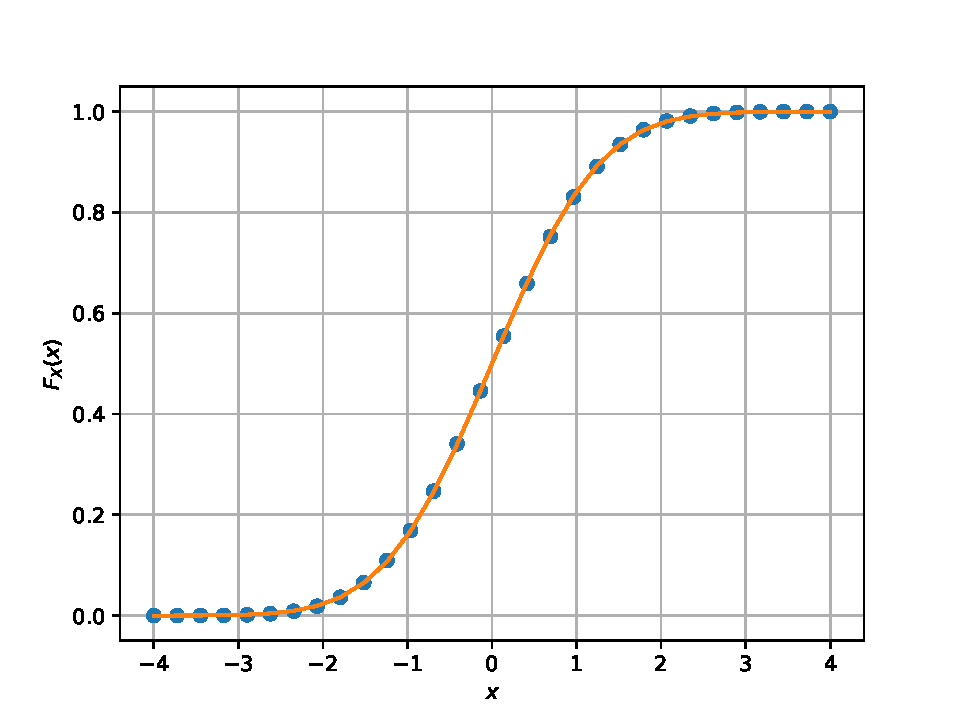
\includegraphics[width=\columnwidth]{./figs/gauss_cdf.pdf}
	\caption{}
	\label{fig:2.2}
\end{figure}

\textbf{2.3: } Load gau.dat in python and plot the empirical PDF of $X$ using the samples in gau.dat. The PDF of $X$ is defined as
\begin{align}
p_{X}(x) = \frac{d}{dx}F_{X}(x)
\end{align}
What properties does the PDF have?

    \solution
    
Download the following files,
\begin{lstlisting}
wget https://github.com/Anshul-Sangrame/AI1110/blob/main/Assignment/solution/2/2_3.py
\end{lstlisting}

Execute the above file using code,
\begin{lstlisting}
python3 2_3.py
\end{lstlisting}

Plot \ref{fig:2.3} obtained is symmetric about y-axis
\begin{figure}[!ht]
    \centering
    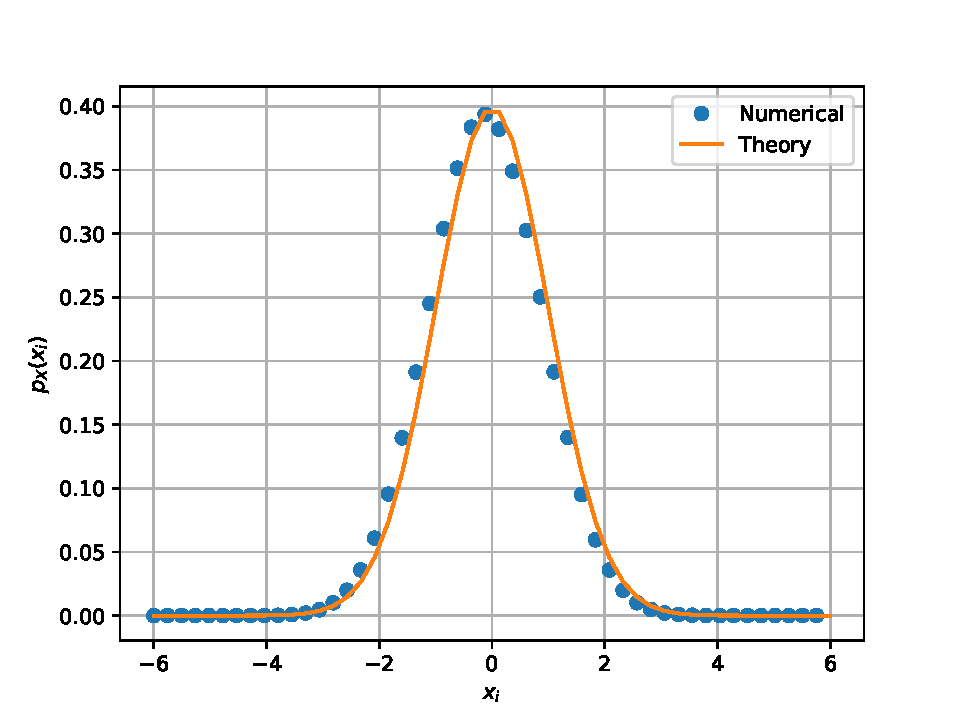
\includegraphics[width=\columnwidth]{./figs/gauss_pdf.pdf}
    \caption{}
    \label{fig:2.3}
\end{figure}

\textbf{2.4: }Find the mean and variance of X by writing a C program.

    \solution
    
Download the following files,
\begin{lstlisting}
wget https://github.com/Anshul-Sangrame/AI1110/blob/main/Assignment/soltion/1/coeffs.h
wget https://github.com/Anshul-Sangrame/AI1110/blob/main/Assignment/solution/2/2_4.c
\end{lstlisting}

Execute the above files using code,
\begin{lstlisting}
gcc 2_4.c -lm
./a.out
\end{lstlisting}
The result is,
\begin{align}
    E\sbrak{U} &= 0.000294 \\
    \text{var}\sbrak{U} &= 0.999561
\end{align}

\textbf{2.5: }Given that 
\begin{align}
p_{X}(x) = \frac{1}{\sqrt{2\pi}}\exp\brak{-\frac{x^2}{2}}, -\infty < x < \infty,
\end{align}
repeat the above exercise theoretically.

    \solution
    
\begin{align}
E\sbrak{U} &= \int_{-\infty}^{\infty} up_X(u) du \\
\end{align}
$up_X(u)$ is a odd function.
\begin{align}
E\sbrak{U} &= 0 \\
\end{align}

\begin{align}
E\sbrak{U^2} &= \int_{-\infty}^{\infty} \frac{u^2}{\sqrt{2\pi}}\exp\brak{-\frac{u^2}{2}} du \\
&= \frac{1}{\sqrt{2\pi}} \int_{-\infty}^{\infty} u\brak{u\exp\brak{-\frac{u^2}{2}}}du
\end{align}

Using integration by parts,
\begin{align}
E\sbrak{U^2} &= \frac{1}{\sqrt{2\pi}} \int_{-\infty}^{\infty} \exp\brak{-\frac{u^2}{2}}du \\
E\sbrak{U^2} &= \frac{\sqrt{2\pi}}{\sqrt{2\pi}} = 1
\end{align}

Hence,
\begin{align}
\text{var}\sbrak{U} &= E\sbrak{U^2} - \sbrak{E\sbrak{U}}^2 \\
&= 1
\end{align}
	
\section{From Uniform to Other}

\textbf{3.1: }Generate samples of 
%
\begin{equation}
V = -2\ln\brak{1-U}
\end{equation}
%
and plot its CDF. 

    \solution
    
Download the following files,
\begin{lstlisting}
wget https://github.com/Anshul-Sangrame/AI1110/blob/main/Assignment/solution/coeffs.h
wget https://github.com/Anshul-Sangrame/AI1110/blob/main/Assignment/solution/3/3_1.c
wget https://github.com/Anshul-Sangrame/AI1110/blob/main/Assignment/solution/3/3_1.py
\end{lstlisting}

Execute the above files using code,
\begin{lstlisting}
gcc 3_1.c -lm
./a.out
python3 3_1.py
\end{lstlisting}

Plot \ref{fig:3.1} is obtained
\begin{figure}[!ht]
    \centering
    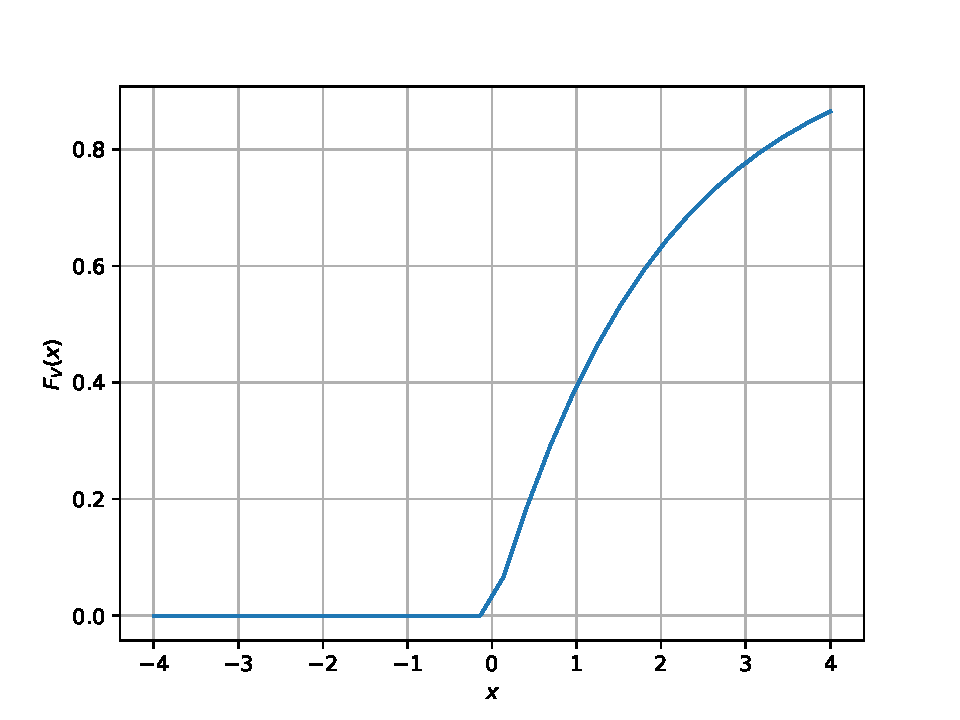
\includegraphics[width=\columnwidth]{./figs/V_cdf.pdf}
    \caption{}
    \label{fig:3.1}
\end{figure}

\textbf{3.2: }Find a theoretical expression for $F_V(x)$.

    \solution
    
\begin{align}
    F_V(x) &= Pr\brak{V \leq x} \\
    &= Pr\brak{-2 \ln \brak{1-U} \leq x} \\
    &= Pr\brak{U \leq 1 - e^{-\frac{x}{2}}} \\
    F_V(x) &= F_U\brak{1 - e^{-\frac{x}{2}}} \\
    &= \begin{cases}
    0, & 1 - e^{-\frac{x}{2}}< 0 \\
    1 - e^{-\frac{x}{2}}, & 1 - e^{-\frac{x}{2}}\in [0,1] \\
    1, & 1 - e^{-\frac{x}{2}}> 1
    \end{cases}
\end{align}

Now,
\begin{align}
    1 - e^{-\frac{x}{2}} &< 0 \\
    \implies x &<0
\end{align}

\begin{align}
    0\leq1 - e^{-\frac{x}{2}} &\leq1 \\
    \implies x &\geq0
\end{align}

\begin{align}
    1<1 - e^{-\frac{x}{2}} \\
    \implies x \in \phi
\end{align}

Hence,
\begin{align}
    F_V(x) = \begin{cases}
    0, & x<0\\
    1 - e^{-\frac{x}{2}}, & x\geq0
    \end{cases}
\end{align}

\end{document}
